En esta seccion se detalla el diseño del sistema. Primero haremos una
descripción y justificación de las grandes decisiones arquitéctonicas
tomadas, para luego hacer una descripción más detallada del sistema
entregado.

\subsection{Minilanguage como DSL interna}
Finalmente la DSL se ha implementado por medio de una DSL~interna en
JRuby. Discutiremos las características de las DSL~internas y las
DSL~externas, así como la razón para elegir JRuby.
\subsubsection{DSL internas}
Definición, ventajas, incovenientes, \ldots{}
\subsubsection{DSL externas}
Definición, ventajas, incovenientes, \ldots{}
% JavaCC, ANTLR
\subsubsection{¿Por qué DSL interna?}
\subsubsection{Ruby y JRuby}
\subsubsection{Sintaxis}
\subsubsection{Ejemplos}

\subsubsection{Inyección código malicioso}
Se ha empleado una sandbox, Java Security Architecture, \ldots{}
\subsubsection{Timeouts}
\subsubsection{Manipulación estado intérprete}

\subsection{Servicio sigue estilo arquitectónico REST}
Explicar REST y justificar su uso.
\subsubsection{JAX-RS}
Bla\ldots

\subsection{MongoDB como Sistema Almacenamiento}
\subsubsection{Opciones valoradas}
\subsubsection{MongoDB}
\subsubsection{Razón elección}

\subsection{Arquitectura Backend}
\subsubsection{Embarrassingly parallel}
http://en.wikipedia.org/wiki/Embarrassingly\_parallel
\subsubsection{Descripción Arquitectura}
\subsubsection{Mover partes aplicación a otros nodos}

\subsection{Clojure como lenguaje de programación}
Características, razón elección, \ldots{}
\subsubsection{Librerías Empleadas}
\begin{description}
\item{CongoMongo} es \ldots{}
\item{Lamina} es\ldots{}
\item{Aleph} es\ldots{}
\item{Gloss} es\ldots{}
\end{description}

\subsection{DARE como procesos sin estado}
http://www.12factor.net/port-binding
http://www.12factor.net/processes
Hablar de por qué se eligió Jetty en vez de Glassfish. Por qué modo
embebido.

\subsection{Librería para Python}
\subsubsection{httplib2}
% rest.py a fondo?
\subsection{Interfaz Línea Comandos en Python}

\subsection{Componentes}
A continuación veamos una visión general del proyecto desde el punto
de vista de un diagrama de componentes UML. En el se muestran los
componentes presentes y las relaciones entre los mismos. A mayores
vamos a realizar una breve descripción de cada uno de ellos:

\begin{description}

\item[minilenguaje:] Es el componente que implementa la DSL definida
  por el proyecto. Este lenguaje se ha denominado minilenguaje. Es
  responsable de transformar la DSL en el formato XML entendido por
  \emph{aAUTOMATOR Runtime}\footnote{Está contenido dentro del
    artefacto \emph{StringEditor}}. Está implmentado en JRuby y
  Java. La parte en JRuby se encarga de definir una DSL interna y la
  parte Java ofrece una API a la misma.
\item[DARE-domain:] Define un modelo de dominio del sistema. Facilita
  una comprensión conceptual del sistema, abstrayéndonos de otras
  consideraciones. Contiene clases como Robot, ExecutionResult y
  PeriodicalExecution. Instancias de estas clases son creadas cuando
  se obtienen datos del sistema de almacenamiento. Está implementado
  en Java.
\item[DARE-war:] Es una aplicación web Java. Contiene todos los
  componentes dentro del recuadro servicio. Puede ser desplegado en
  cualquier servidor de aplicaciones JEE y/o contenedor de servlets.

  Siguiendo el patrón MVC\footnote{Modelo Vista Controlador} este
  modelo es el responsable de la parte de vista y controlador. Utiliza
  la api JAX-RS para lleva a cabo esta labor. Utiliza a DARE-domain
  como modelo y DARE-backend ofrecería servicios de persistencia y
  ejecución.

  Este componente ha sido concebido de modo que se puede desplegar en
  varios nodos, ya que se sigue una filosofía
  \emph{share-nothing}. Para ellos nos hacemos valer de las
  características sin estado de REST. Es decir, podemos tener varios
  servidores web ejecutándose en distintos nodos. Está implementado en
  Java.

\item[DARE-backend:] Es el componente encargado de comunicarse con la
  base de datos MongoDB tanto para leer como para escribir los objetos
  definidos en DARE-domain. Recibe también las peticiones de ejecución
  para aAUTOMATOR. Luego utilizando la parte cliente de DARE-workers
  las reparte entre los procesos \emph{worker} que se están
  ejecutando.

\item[DARE-workers:] Este componente está compuesto por una parte
  cliente que lanza peticiones de ejecución a aAUTOMATOR. La parte
  servidor, de ahora en adelante \emph{worker}, interpreta esas
  peticiones y hace el trabajo correspondiente. Uno o varios de estos
  workers pueden estar lanzados en función de las necesidades de
  escalabilidad y fiabilidad necesarios.

  Cada worker es un proceso por lo que alguno de ellos podría dejar de
  funcionar y DARE podría seguir ofreciendo su servicio. Además al ser
  cada uno un proceso se pueden ejecutar localmente en el mismo nodo o
  repartirlo a traves de varios nodos del cluster. La parte cliente es
  capaz de descubrirlos y repartir la carga de peticiones entre los
  workers. Aparte comprueba continuamente el estado de salud de los
  workers para que el servicio continúe funcionando aun en la
  presencia de errores en los workers.

 Tanto la parte servidor como cliente están implementados en Clojure.

\item[DARE-util:] Es un cajón de sastre donde se encuentran diversas
  funciones de utilidad usadas por varios otros módulos.

\item[DARE-web:] Este módulo se utiliza para facilitar el despliegue
  de la aplicación. Toma el fichero \emph{war} con la aplicación y lo
  ejecuta creando un servicio web. Para ello emplea el contenedor de
  servlets embebido, Jetty\cite{JETTY}. Jetty es un contenedor de
  servlets ligero, por lo que es especialmente adecuado para lanzar
  numerosas instancias de la aplicación. Este componente está
  implementado en Clojure.

\item[DARE-java:] %TODO extract
\item[DARE-python:] Este módulo implemente la librería cliente para
  Python, así como la aplicación de línea de comandos. Como se ha
  descrito anteriormente usa httplib2 para llevar a cabo la
  comunicación con el servicio.

  La aplicación de línea de comandos está contenida en este componente
  y utiliza la librería creada para llevar a cabo su
  funcionalidad. Como es lógico está implementado en Python.
\end{description}

\begin{landscape}
\begin{figure}[p]
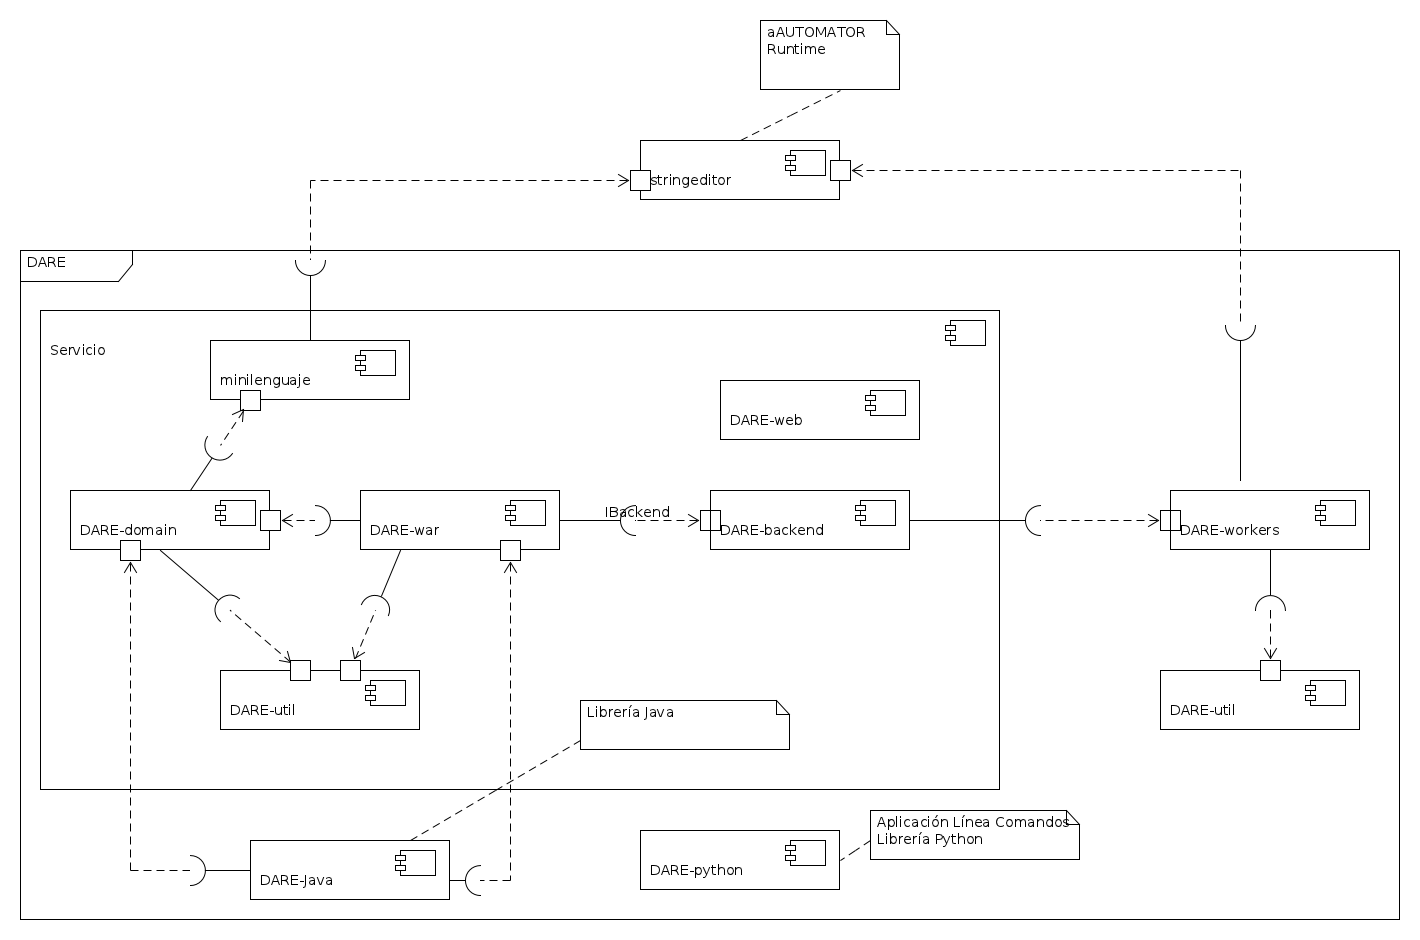
\includegraphics[width=1.4\textwidth]{chapters/technical-manual/diagrams/diagrama_componentes.png}
\caption{Diagrama Componentes DARE}\label{diagrama_componentes_dare}
\end{figure}
\end{landscape}


\subsubsection{Diagrama clases minilenguaje}

\subsubsection{Descripción Implementación transformer.rb}
Descripción general \ldots{}
% transformer.rb en modo literario

\subsubsection{Diagrama clases DARE-war}
\begin{figure}[!hbp]
\makebox[\textwidth]{\framebox[5cm]{\rule{0pt}{5cm}}}
\caption{Diagrama dominio}
\end{figure}

\subsubsection{Diagrama clases DARE-backend}
% a fondo backend/core.clj?
\subsubsection{Diagrama clases DARE-workers}
% a fondo workers/client.clj, workers/server.clj?

\subsubsection{Esquema datos Sistema Almacenamiento}
